\section{Our Modeling Methodology}
\label{sec:model}
\vspace{10pt}

In this section, we describe the general performance modeling ideas we employ in our research. In Section~\ref{sec:eval}, %we describe how 
we adapt this basic model to our three application case studies whose performance we study on the Amazon EC2 cloud. 

Our interest is in interactive data-serving applications whose %server applications, the 
performance is typically %can be 
characterized in terms of their throughput (request/s) and average request response time or latency.  %(duration of each request).  
 It is important to note that our primary interest in this paper is {\em not in identifying the most accurate performance model but rather in exploring if diversity in the VMs used for calibrating our chosen model helps improve its efficacy}. 
Therefore, although numerous modeling choices exist in the literature for such applications (see Section~\ref{sec:related}), we choose a relatively simple approach based on multiple linear regression because: (i) it serves as a good starting point for evaluating our hypothesis, (ii) it is easy to cast, train, and evaluate, and (ii)it  works well - especially under low/moderate throughputs which we expect to be normal operating regions for well-provisioned, performance-sensitive tenant workloads -  as demonstrated in past work~\cite{Stewart07,Kelly:2005:DPA:1251522.1251530}. 

%For low rates of throughput, the latency is nearly constant and increases slowly with increasing throughput.  As throughput approaches the maximum capacity of the server, the latency increases much more rapidly.  For our study, we study the low-throughput region, which is approximately linear for a variety of VM instances, applications, and throughputs.  Therefore a multiple linear regression is justified.

\begin{itemize}
\item Section 3.1: Background on Multi-Linear Regression. Describe basics from a standard source and cite it. Summarize the main assumptions underlying regression. Cite papers that have used linear regression based modeling for data center/cloud workloads. 
\item Section 3.2: Our Model. Describe what we wish to predict. Describe what all our input variables could be. Describe what subset we choose. Make a note about possible positive correlation between num cores and memory (refer to Figure 2). Describe what metric (predicted R-2) we use for measuring the efficacy of our model. 
\item Section 3.3: Discuss implications of lack of independence between num cores and memory. Discuss what operating regions our model is likely to capture well and which ones it might not. Discuss possible extensions. Point to related work for discussion of alternate modeling approaches that have been explored. Discuss possible problems with using predicted R-2 as a measure of model accuracy and alternative metrics (e.g., in Chris Stewart's paper). 
\end{itemize}

%\subsection{Background on Multiple Linear Regression}
\noindent{\bf Multiple Linear Regression:} Given a data set \\ $\{y_i,x_{i1},\ldots,x_{ip}\}^n_{i=1}$, a linear regression on multiple independent variables $x_{p}$ and dependent variable $y$ is a set of parameters $\beta_i$ that model a linear relationship between $y$ and $x_{i}$~\cite{CMUStatsBook}.

\begin{displaymath}{
y_i = \beta_1 x_{i1}+\ldots+\beta_{p}x_{ip}+\epsilon_i
}\end{displaymath}

The parameters $\epsilon_i$ are the error terms, an unobserved random variable.  The parameters $\beta_i$ are chosen to minimize the values of $\epsilon_i$ for the entire data set.  Specifically, the $\beta_i$ are chosen to minimize the sum of squares $\sum_{i=1}^{n} \epsilon^2_i$.

%\subsection{Model}
%Our goal is to model the performance of different virtual machine instance types, and show a correlation between the performance of those applications that can be used to predict the performance of those applications on new virtual machine instance types.

%The performance of a server application is evaluated as the time latency $y_{L}$ for responding to a request.  
We choose as our dependent variable the average latency $y_{L}$ and as our independent variables: (i) workload/application properties - throughput, degree of replication, and read/write ratio and (ii) resource capacity of the VMs being used - number of CPU cores, clock rate of each CPU, memory, network bandwidth, and type of storage (SSD vs. magnetic). 
%is the dependent variable in our model.  The benchmarks are run at multiple levels of throughput (requests/second), which is taken as an independent variable $x_{T}$

%Virtual machine instances vary by in many ways:  the type of CPU, CPU clock speed, number of CPUs, amount of memory, type or storage (SSD vs magnetic), amount of storage, and available network bandwidth.  Each of these parameters can be modeled by as an independent variable $x_p$.

We define a training set $S = \{VM_i\}^n_{i=1}$ as a set of virtual machines, each characterized by $x_p$.  In each of our experiments, we run the application whose performance we wish to model on  $VM_i$ for various $x_{T}$ and measure the latency $x_{L}$.  We then find a multiple linear regression $M_S$ on $\{y_{iL},x_{iT},\ldots,x_{ip}\}^n_{i=1}$.  (For a given instance $VM_i$, the values of $x_{ip}$ are fixed for all measurements for that instance.) 

%We then consider another instance $VM_{test}\notin S$ and use $M_S$ to predict the dependent variable $y_L$.

\begin{figure}
    \centering
    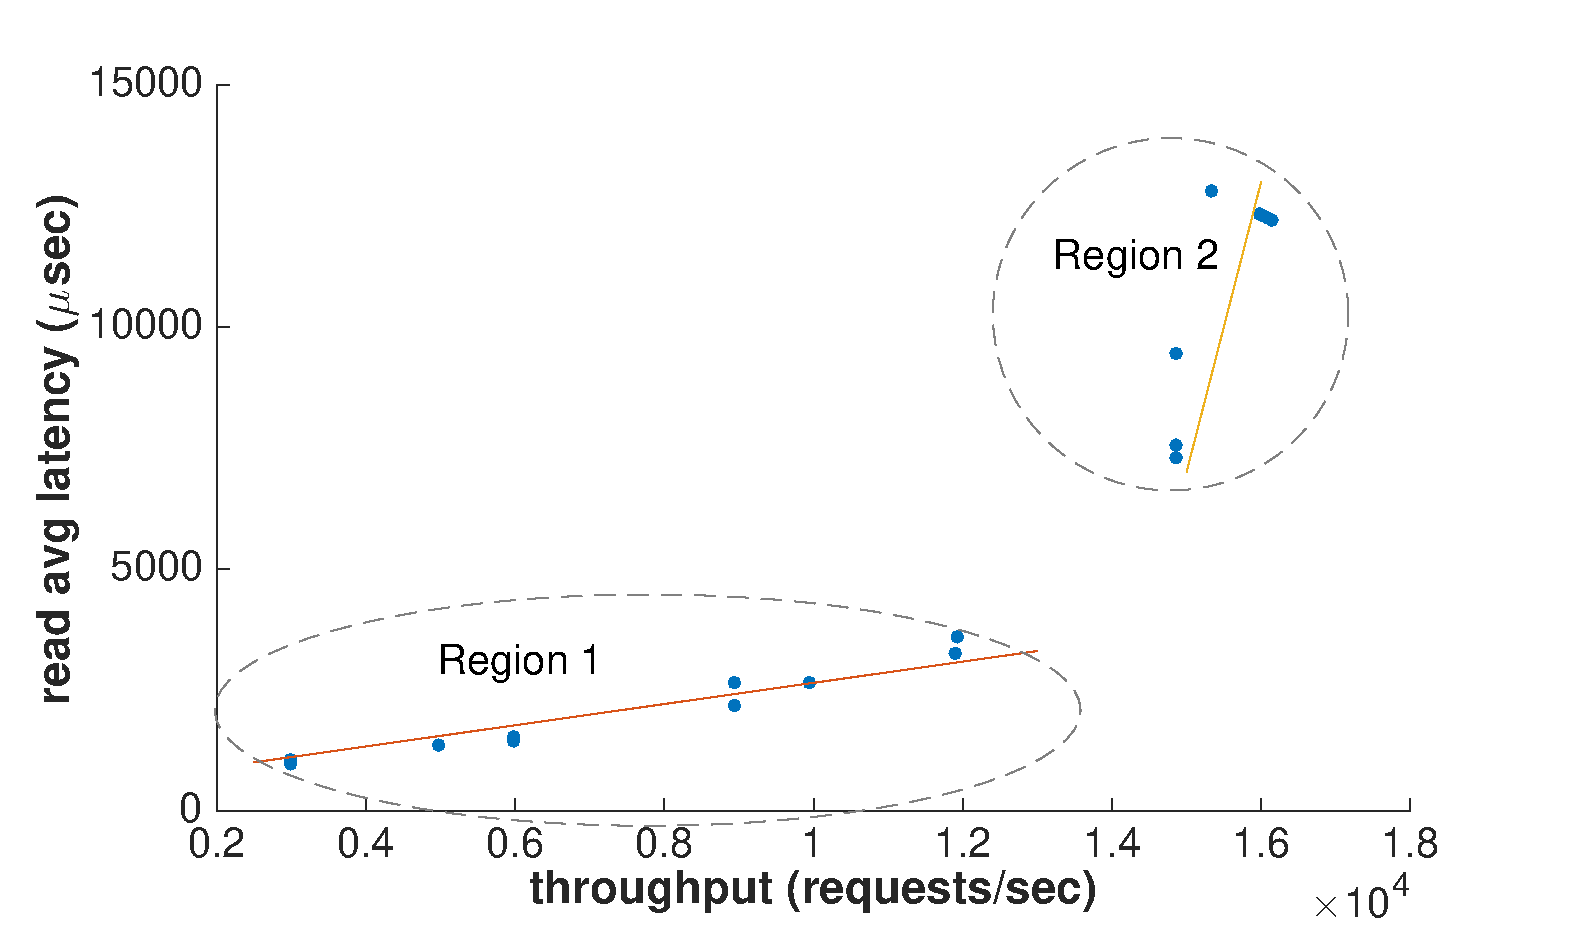
\includegraphics[scale = 0.35]{two_regions.eps}
    \caption{Two regions of latency vs. throughput for Redis. }
    \label{figure:combined}
\end{figure}

\noindent{\bf Measure of Model Efficacy:} We use the predicted coefficient of multiple determination ($R^2_{predicted}$) as our measure of model accuracy which is defined as: 
\theoremstyle{definition}
\newtheorem{mydef}{Definition}
\begin{mydef}
For a test instance $VM_{test}$ with $x_{test,i}$,
\begin{displaymath}
R_{predicted}^2=1-\frac{\sum_{i=1}^{n} (y_{test,i} - \hat{y}(x_{test,i}))^{2}}{\sum_{i=1}^{n} (y_{test,i} - \bar{y_{test}})^{2}}
\end{displaymath}
where
\begin{displaymath}
\hat{y}(x_{test,i})=\sum_{i=1}^{n} \beta_i x_{test,i}
\end{displaymath}
and $\bar{y}_{test}$ is the mean of $y_{test,i}$.
\end{mydef}

%\subsubsection{Input and Predicted Variables}

To see evidence supporting our hypothesis, we expect to see the following behavior: for larger training sets $S$, the model should fit better to $VM_{test}$, corresponding to an increasing $R^2_{predicted}$, assuming sufficient variability in the values of $x_p$ for $VM_j\in S$ to cover the values of $x_p$ for $VM_{test}$.  

\noindent{\bf Discussion:} Our linear regression based model is known to perform poorly when queueing delays become dominant contributors to overall latency~\cite{Stewart07}. 
For example, if we were to model the entire set of latency observations (for experiements done using Redis, more details
in Section~\ref{sec:redis}) using our model, we would obtain a poorer predictor than the two separate linear regression
models shown in Figure~\ref{figure:combined}, one each for the ``low/moderate'' (Region 1) and ``high'' (Region 2) throughput regions. This suggests two points: (i) using domain knowledge (e.g., the distinction between low and high throughput regions), a 
tenant may be able to use linear regression to obtain better models, and (ii) more sophisticated models may be 
warranted for the needs of certain tenants. Again, since our interest is in the impact of diversity on modeling accuracy,
we focus only on modeling performance in Region 1 for the rest of this paper. 

It is important to keep in mind the basic assumption of linear regression about the independent variables being independent of each other (i.e., the $x_p$ for $VM_j\in S$ need to be independent). Interestingly, among the independent
variables in our model, the number of cores and memory capacity are prone to be problematic on this front - typically
larger VMs come both with more CPUs and more memory - see Figure~\ref{fig:diversity}. To overcome this problem, we attempt to choose VM types
in our experiments where this correlation is weak. Furthermore, the results we present in this paper are for a subset
of our experimental findings wherein the entire working set fits in VM memory, rendering memory moot as a predictor of
performance (we do incorporate memory in our more general experiments). Finally, the potential shortcomings of predicted 
$R^2$ as a measure of model accuracy should be kept in mind when interpreting our results~\cite{CMUStatsBook}. 
%}
  
%\subsubsection{Measure of Model Efficacy}  
  
%\subsection{Discussion}
%\vspace{10pt}

